\documentclass[10pt,a4paper]{article}

\usepackage[T1]{fontenc}
\usepackage[utf8]{inputenc}
\usepackage{helvet}
\renewcommand{\familydefault}{\sfdefault}
\usepackage[margin=18mm,top=20mm,bottom=20mm]{geometry}
\usepackage{xcolor}
\usepackage{graphicx}
\usepackage{booktabs}
\usepackage{tabularx}
\usepackage{longtable}
\usepackage{enumitem}
\usepackage{titlesec}
\usepackage{tcolorbox}
\usepackage{microtype}
\usepackage{pdflscape}
\usepackage{fancyhdr}
\usepackage[hidelinks]{hyperref}
\tcbuselibrary{skins,breakable}

\definecolor{qink}{HTML}{14110E}
\definecolor{qorange}{HTML}{E05A28}
\definecolor{qorangelt}{HTML}{FBE7DC}
\definecolor{qcream}{HTML}{FBF7F1}
\definecolor{qgrey}{HTML}{6B6560}
\definecolor{qline}{HTML}{C9C2B8}
\definecolor{qblue}{HTML}{1F5F8B}
\definecolor{qbluelt}{HTML}{DCE8F1}
\definecolor{qgreen}{HTML}{2F6B4F}

\color{qink}
\setlength{\parindent}{0pt}
\setlength{\parskip}{5pt}
\linespread{1.06}

\titleformat{\section}{\color{qorange}\large\bfseries}{\thesection.}{0.5em}{}
\titleformat{\subsection}{\color{qink}\normalsize\bfseries}{\thesubsection}{0.5em}{}
\titleformat{\subsubsection}{\color{qink}\small\bfseries}{}{0em}{}
\titlespacing{\section}{0pt}{16pt}{6pt}
\titlespacing{\subsection}{0pt}{11pt}{3pt}

\setlist[itemize]{leftmargin=14pt,itemsep=2pt,topsep=3pt,parsep=0pt}
\setlist[enumerate]{leftmargin=16pt,itemsep=2pt,topsep=3pt,parsep=0pt}

\newtcolorbox{callout}[1][]{colback=qcream,colframe=qline,boxrule=0.5pt,arc=2pt,
  left=7pt,right=7pt,top=6pt,bottom=6pt,breakable,#1}
\newtcolorbox{moment}[1][]{colback=qorangelt,colframe=qorange,boxrule=1pt,arc=2pt,
  left=7pt,right=7pt,top=6pt,bottom=6pt,breakable,#1}
\newtcolorbox{elasticbox}[1][]{colback=qbluelt,colframe=qblue,boxrule=0.7pt,arc=2pt,
  left=7pt,right=7pt,top=6pt,bottom=6pt,breakable,#1}

\newcommand{\gy}[1]{{\color{qgrey}#1}}
\newcommand{\code}[1]{{\small\texttt{#1}}}
\newcommand{\lead}[1]{{\color{qgrey}\small #1}}

\pagestyle{fancy}\fancyhf{}
\renewcommand{\headrulewidth}{0.4pt}
\renewcommand{\headrule}{\hbox to\headwidth{\color{qline}\leaders\hrule height \headrulewidth\hfill}}
\lhead{\small\color{qgrey}Quota \textbullet{} an autonomous commissions desk}
\rhead{\small\color{qgrey}CalHacks 2026 \textbullet{} Hyphenate track}
\cfoot{\small\color{qgrey}\thepage}

\begin{document}

%==================================================================
\begin{center}
{\color{qorange}\Huge\bfseries Quota}\\[5pt]
{\large An autonomous commissions desk.}\\[10pt]
{\color{qgrey}\small CalHacks 2026 \ \textbullet\ \ Hyphenate: \emph{The Hyphenated Enterprise \textemdash{} Autonomous Systems for Finance}}\\[2pt]
{\color{qgrey}\small Also entered in Elastic's \emph{Find the Signal with Elasticsearch} challenge}\\[8pt]
{\small\href{https://github.com/aaditisinghal/Quota}{\texttt{github.com/aaditisinghal/Quota}} \ \textbullet\ \ 18{,}050 lines of Python, 4{,}734 of TypeScript, 284 tests, 66 commits}
\end{center}

\vspace{4pt}
\begin{moment}
\textbf{The one line you asked for, on the seats it fills}\\[3pt]
Quota fills the \textbf{commissions analyst} and \textbf{deferred-commission accountant} seats at a SaaS company: it drafts every commission line, every payout file and every ASC 340-40 journal entry, and it approves none of them.
\end{moment}

\vspace{2pt}
\section*{\color{qink}The evidence, up front}
\vspace{-6pt}
\lead{Your four questions, answered in one block. Every number below is measured by a command in the repo, and every section that backs one is named.}

\vspace{4pt}
\renewcommand{\arraystretch}{1.25}
\begin{tabularx}{\textwidth}{@{}p{34mm}X@{}}
\toprule
\textbf{Is it real enough?} &
A six-month simulated world with 20 reps, $\sim$245 deals and $\sim$1{,}500 events, carrying \textbf{16 kinds of planted error with a written answer key}. On a \textbf{held-out seed} it caught \textbf{40 of 40} planted cases with \textbf{0 false flags} and \textbf{0 wrong automatic payouts}. Billing is real: the same run against a \textbf{Stripe sandbox} produced 241 invoices, 210 card payments and 3 refunds totalling \$214{,}916.66, and every one of 454 billing rows carries its Stripe id. The capitalization policy is lifted from \textbf{three public 10-K filings}. \hfill\gy{\S4}\\
\textbf{Would you hire it?} &
Two seats, each with a named capability set. Neither can approve anything, and the write path refuses when they try: \code{NO\_CAPABILITY, INV5\_SELF\_APPROVAL, INV5\_WRONG\_APPROVER}, logged as refusal \code{R-0001}. Every write passes \textbf{seven invariants}; every number traces to the row, rule and person behind it; \textbf{580 of 580 decisions replay exactly} from their recorded inputs. \textbf{94.9\%} of lines go straight through, at \textbf{0.7 escalations per 100 events}. \hfill\gy{\S2, \S5}\\
\textbf{Did we see\newline something new?} &
Commissions \textemdash{} the one finance object that is simultaneously a payroll liability, a capitalized asset under ASC 340-40, a legal obligation under state wage law, and an argument with a salesperson. Nobody has made it autonomous. Two things inside it are new on their own: a \textbf{semantic sweep of sales email that holds a payout} when a rep promised something the contract never said, and an \textbf{onboarding path through a real HR web app's screens} rather than its API. \hfill\gy{\S6}\\
\textbf{The moment} &
A rep's own email, to a customer, with no shared words with any contract term, holds \$6{,}000 out of payroll and warns the Controller that revenue may be wrong too. Then a rep claims a deal closed four days earlier than it did, and Quota refuses him twice, routes him to his VP, refuses the VP for exceeding a \$5{,}000 limit, and refuses \emph{itself} when asked to approve the result. \hfill\gy{\S1}\\
\bottomrule
\end{tabularx}

\vspace{8pt}
\begin{callout}
\textbf{Where the ninety seconds go, if that is all there is.} \code{python -m quota serve} opens on \textbf{Home}: the money pending, cleared and held, the six inputs it reads, and everything waiting on a person. Click Riley Shah $\to$ the held Summit line $\to$ the evidence card: the sentence the rep wrote, the search that found it, the two code checks that kept it. Then \textbf{Case}: Jordan's dispute, the struck-through CRM date, the countersignature that beats it, and four refusals in a row. Then press \code{Ctrl-K} and \textbf{hand over the keyboard}.
\end{callout}

\clearpage
%==================================================================
\section{The moment}

\lead{Hyphenate asks for the moment the system catches what others missed, recovers from something going wrong, or defends a decision when questioned. We have one of each. The video opens with the first.}

\subsection{It catches what no one would have caught}

Riley Shah closed Summit Dental. The signed contract has no early-exit clause, the CRM is clean, the invoice is paid, and every number in the ledger agrees with every other number. On any reconciliation-based system, this deal is finished.

Five days later Riley wrote to the customer:

\begin{moment}
\textit{``Between us, if your team hasn't adopted it by end of Q3 we'll let you out of year two, no penalty. Don't worry about the paperwork.''}\\[3pt]
\gy{\code{MSG-SIDE-0001}, subject ``Re: rollout plan'', sent 2026-05-05, account Summit Dental, \code{side\_letter.jsonl} row 1.}
\end{moment}

That sentence contains no shared vocabulary with ``termination'', ``cancellation'' or ``clause''. Keyword search does not find it; measured, BM25 finds \textbf{5 of 12} planted promises in a 2{,}940-message corpus. Semantic search over Elastic finds it at rank 1 and \textbf{10 of 12} overall.

Finding it is not the hard part. Believing it is. So Quota does three things in order, and only the first involves a model:

\begin{enumerate}
\item A model reads the one message and reports whether the sender promised the customer a benefit, of which kind, \textbf{in which exact words}.
\item \textbf{Code} checks that those exact words appear in the message body, whitespace-normalised. A quote the model invented is discarded. A hallucination cannot hold anyone's money.
\item \textbf{Code} checks the signed contract. If the contract already grants what was promised \textemdash{} a termination-for-convenience window long enough, a price-increase cap \textemdash{} the message is \code{covered}, and nothing happens.
\end{enumerate}

Summit's contract grants none of it. So Quota wrote decision \code{D-0014}: outcome \textbf{held}, \textbf{\$6{,}000.00}, reason \code{OFF\_CONTRACT\_COMMITMENT}, and opened \code{A-0009}, a commitment review, for Priya Nair, the Controller. Riley's line is out of the May payroll file until she answers. The Controller is also told that \emph{revenue} may be misstated, because an undisclosed exit right changes the contract term the revenue schedule is built on.

That is a commissions agent telling a Controller her revenue might be wrong, because of an email.

\subsection{It defends a decision, four times over}

End of April. Jordan Kim sold Acme a \$120{,}000, 36-month contract and wants it in Q1, where his rate is 1.5$\times$.

\begin{callout}
\small
\textbf{1.} Jordan: \emph{``Acme closed Mar 31.''} \ \ Quota \textbf{holds} and shows its work: the CRM says Mar 31 \gy{(struck through)}; the e-signature log says \textbf{countersigned Apr 2, 10:14 AM Pacific}; rule \code{R-BOOKING-01} says a deal books on countersignature. \textbf{\$12{,}000.00, not \$18{,}000.00 \textemdash{} a \$6{,}000.00 difference.}\\[4pt]
\textbf{2.} Jordan pushes again with no new evidence. Held again, and told exactly that. He types \code{escalate}.\\[4pt]
\textbf{3.} Marcus Lee, VP Sales Ops, approves the exception. His limit is \textbf{\$5{,}000}. Approval \code{A-0001} is recorded \emph{and} routed onward as \code{A-0002} to the Controller, because an approval over a limit is not an approval.\\[4pt]
\textbf{4.} Someone asks the commissions seat to approve \code{A-0002} itself. The write path refuses and logs \code{R-0001}: \code{NO\_CAPABILITY}, \code{INV5\_SELF\_APPROVAL}, \code{INV5\_WRONG\_APPROVER}.\\[4pt]
\textbf{5.} Priya approves. That records precedent \code{P-0001}, and \code{CL-0002} books \$18{,}000 in Q1, superseding \code{CL-0001} \textemdash{} by appending, not by editing.
\end{callout}

Four refusals, each with a code, each a numbered row anyone can look up later. The agent never argues from opinion; it argues from a timestamp.

\subsection{It recovers from something going wrong \textemdash{} including from itself}

\textbf{The business failure.} In June, Acme churns and gets \$90{,}000 back. One event moves eight numbers at once: deferred revenue, cash, the customer balance, the forecast, Jordan's commission, the deferred-commission asset, commission expense and attainment. Quota claws back \$18{,}000, writes off \$16{,}500 of unamortized deferred commission, and books \$1{,}500 that had already amortized. Every invariant stays green and the trial balance still balances.

Jordan is in California, and his signed plan makes commissions advances until earned, so the \$18{,}000 becomes a receivable in account \textbf{1290} and is recovered from his \emph{next} commissions \textemdash{} oldest recovery first, never by billing him. Had he already left, Quota would stop and ask the Controller instead.

\textbf{Our own failure.} During the live Elastic rehearsal, the auditor agent answered a question about Marcus's approvals with one wrong clause: it said he had approved an exception ``for himself''. He had not. The fault was ours \textemdash{} the decision mirror had taken Marcus's grant message as the rep. We found it because \code{quota elastic verify} rebuilds every mirrored document from the ledger and compares it, so drift is loud. The mirror now names a rep only for an AE. \textbf{The wrong answer is still printed in the repo}, in \code{docs/ELASTIC\_LIVE.md} and in Figure 3 of this document, because a system that only publishes its wins is not an audit trail.

%==================================================================
\section{The seats, and the limits that come with them}

\subsection{What each seat may do}

Each seat is a principal with an explicit capability set. There is no admin account, no bypass, and no capability that means ``everything''.

\renewcommand{\arraystretch}{1.2}
\begin{tabularx}{\textwidth}{@{}p{42mm}X p{30mm}@{}}
\toprule
\textbf{Principal} & \textbf{May do} & \textbf{Limit}\\
\midrule
\code{seat:commissions\_analyst} & \code{read:*}, draft commission lines, draft approval requests, draft messages, draft payroll files, record decisions, claim events & \gy{approves nothing}\\
\code{seat:deferred\_accountant} & \code{read:*}, draft journal entries, draft messages, record decisions, claim events & \gy{approves nothing}\\
\midrule
Jordan Kim \gy{AE} & dispute his own lines, send messages & \gy{own lines only}\\
Marcus Lee \gy{VP Sales Ops} & approve plan exceptions & \textbf{\$5{,}000}\\
Priya Nair \gy{Controller} & approve exceptions, journal entries, payroll files, commitment reviews; lock periods & \gy{none}\\
Grace Liu \gy{CFO} & the same, as backup after 2 business days & \gy{only what is routed to her}\\
Dana Ortiz \gy{Payroll} & release a payroll file & \gy{release only}\\
\code{salesops.bot} \gy{automated colleague} & \textbf{nothing} \gy{\textemdash{} it emits half-finished work into the world and Quota has to cope} & \gy{\textemdash}\\
\bottomrule
\end{tabularx}

\vspace{4pt}
Whoever requests cannot approve. A person who is away approves nothing automatically; their work routes to a backup after two business days, and an approver who would personally benefit \textemdash{} credited on the deal, or managing someone who is \textemdash{} is skipped in favour of the Controller.

\subsection{When it asks}

Eight triggers, written down before the code was built, each implemented and each testable:

\begin{enumerate}[label=\textbf{\arabic*.}]
\item \textbf{Sources disagree above materiality} (\$500 or 2\% of the payout). The written source ranking settles it; the decision records that the disagreement was material and what it was worth.
\item \textbf{Authority is needed.} Exceptions, splits and territory go to the VP within \$5{,}000, then the Controller, then the CFO.
\item \textbf{\code{NO\_RULE}.} A clause or currency no rule covers \textemdash{} a ramp, a non-USD contract. No line is written at all; the plan owner is asked.
\item \textbf{Legally sensitive.} Terminations and unsigned plans go to the Controller. A leave of absence becomes a \code{leave\_review} for the Controller and HR, and nothing changes in the meantime.
\item \textbf{An integrity signal.} A close date backdated after a period lock; an approver who would benefit; the same rep needing repeated exceptions.
\item \textbf{A correction into a locked period.} It posts in the open period instead, and reaches the Controller through the entry approval.
\item \textbf{Someone must sign.} Every seat-drafted entry, every payout file, every period lock.
\item \textbf{Its own checks fail.} Before every payroll run Quota re-runs all seven invariants and re-hashes the chain. On any failure nothing is paid and the Controller is told.
\end{enumerate}

\subsection{How sure it is, and why that is not a model's opinion}

Every commission line carries a confidence score. It is \textbf{the weakest of six evidence factors}, times 100 \textemdash{} never a model's self-rating, and never an average, because an average lets five good signals hide one broken one.

\begin{tabularx}{\textwidth}{@{}p{30mm}X@{}}
\toprule
\textbf{Factor} & \textbf{What drops it}\\
\midrule
\code{booking\_date} & another source names a different date; the ranking rule that settled it is named\\
\code{amount} & the CRM and the contract disagree on the base\\
\code{owner\_splits} & \textbf{0} if splits do not sum to 100\%, or nobody owns the deal; 0.8 if the split came from the CRM with no VP record\\
\code{extraction} & the figure is not verbatim in a structured record, or no second source agrees\\
\code{rule\_coverage} & \textbf{0} on \code{NO\_RULE}; 0.9 when only a saved precedent covers it\\
\code{integrity} & capped at \textbf{0.40} by a backdated edit, an off-contract promise, or an approver conflict\\
\bottomrule
\end{tabularx}

\vspace{4pt}
$\geq 90$ clears to the payout file (the Controller still signs the batch). $\geq 70$ clears with a note. Below 70 it is held and the right person is asked. The five factors a decision's own rows can tell are stored \emph{inside the decision}, so a replay reproduces them; integrity is applied later, because backdating is something you learn afterwards. Collection is deliberately not a factor \textemdash{} an unpaid invoice is a hold, shown separately, not a doubt about the arithmetic.

%==================================================================
\section{The company it works in}

\textbf{Fernhill} is a SaaS company that pays salespeople on deals. Its stack is the ordinary one: a CRM, an e-signature log, contract PDFs, an HR system, a billing system, signed commission plans, and a spreadsheet that last quarter's payouts were actually run from.

The cast is five people and one bot. Jordan Kim is an AE who disputes. Marcus Lee is a VP who grants exceptions and sometimes exceeds his limit. Priya Nair is the Controller who says no. Grace Liu is the CFO, and exists mainly to be the backup when Priya is away. Dana Ortiz releases payroll. \code{salesops.bot} is the automated colleague that leaves work half done \textemdash{} it moves half a territory and stops.

The mess is the point. The CRM amount disagrees with the contract. A close date is backdated into a locked quarter. Splits add to 110\%. A manager promises a SPIF in chat that no plan contains. A customer pays 98\% after wire fees. A payroll export differs from the approved lines by \$340. A rep leaves in California mid-quarter. A deal is credited 100\% to two different people.

\begin{callout}
\textbf{Why commissions, personally.} My cofounder's father has run a loan brokerage for thirty years. The lending is not the hard part; paying for it is. He has a large team of telecallers working leads, and \textbf{three people whose entire job is tracking who sold what and what each telecaller is owed}. The first week of every month goes to one argument: who gets paid what. The sales sheet says one thing, the payout sheet says another, and a telecaller says he was promised more over WhatsApp. That last one \textemdash{} the promise that exists only in a message \textemdash{} is the reason \S1.1 exists. Three people, one object, and the same argument every month is also exactly the shape this track asked for: a few seats that work closely together.
\end{callout}

%==================================================================
\section{Is it real enough?}

\subsection{What is real, what is simulated, and how we know}

\renewcommand{\arraystretch}{1.2}
\begin{tabularx}{\textwidth}{@{}p{38mm}p{24mm}X@{}}
\toprule
\textbf{Part} & \textbf{Status} & \textbf{How we know it works}\\
\midrule
Ledger, invariants, hash chain & \textbf{Real}, built here & Invariants run on every write; \code{quota verify} recomputes the chain from genesis and re-hashes every row\\
Calculator, amortization, entries & \textbf{Real}, deterministic & Unit tests against hand-calculated cases: \$12{,}000 vs \$18{,}000 on Acme, 36 $\times$ \$500 amortization, the \$18{,}000 / \$16{,}500 / \$1{,}500 clawback\\
Decisions & \textbf{Real}, replayable & Each records its inputs as \gy{(table, id, version, sha256)}; \code{quota replay D-0005} recomputes it from that as-of view\\
Billing & \textbf{Real with \code{-{}-stripe}} & Stripe sandbox with test clocks; every billing row carries its Stripe id \gy{(\code{in\_...}, \code{pi\_...}, \code{re\_...})}; a duplicate payment webhook is stopped by the mirror's idempotency check before it reaches Stripe\\
HR system & \textbf{Real app}, simulated data & A BambooHR clone running on \code{:8080}; read through its \emph{screens} by a computer-use agent, then verified 100\% against its own API, with its audit log showing zero writes\\
Screens and API & \textbf{Real}, built here & FastAPI + React; \code{tests/test\_e2e\_cfo.py} clicks the whole demo path in a headless Chromium\\
\midrule
CRM, contracts, plans, e-sign & \gy{Simulated, seeded} & \code{quota/sim/generator.py}; facts arrive as events only when the clock reaches them\\
People & \gy{Scripted, rule-played, or model-played} & Scripted in the Acme demo; rule-played in the eval; played by Claude with \code{-{}-live}. They act only through the same chat and approval API, under the same write-path checks\\
Planted errors & \gy{Simulated, with an answer key} & \code{quota eval -{}-seed N} compares every decision to \code{answer\_key.json}\\
\bottomrule
\end{tabularx}

\subsection{The scorecard}

\code{python -m quota eval --seed 7} and \code{--seed 1729}. Twenty reps, January to June 2026, $\sim$245 deals, $\sim$1{,}500 events, 40 planted cases across 16 error types. \textbf{A case counts only when both the outcome and the dollar amount match the key.}

\begin{tabularx}{\textwidth}{@{}Xp{30mm}p{32mm}@{}}
\toprule
\textbf{Metric} & \textbf{Seed 7} \gy{(development)} & \textbf{Seed 1729} \gy{(held out)}\\
\midrule
Planted-error recall & 40 / 40 \gy{(100\%)} & 40 / 40 \gy{(100\%)}\\
False flags & \textbf{0} & \textbf{0}\\
Wrong automatic payouts & \textbf{0} & \textbf{0}\\
Pushback test \gy{(20 scripted disputes)} & held 10/10 invalid, conceded 10/10 valid & same\\
Straight-through rate & 94.7\% & 94.9\%\\
Escalations per 100 events & 0.7 & 0.7\\
Replay match & 100\% \gy{(554 decisions)} & 100\% \gy{(580 decisions)}\\
Write-path refusals & 2, both \code{INV6\_PAYROLL\_MISMATCH} & 2, same\\
\bottomrule
\end{tabularx}

\vspace{4pt}
\textbf{The miss, and what it tells you.} On the first run of held-out seed 1729, one case came back \code{held} where the key said \code{posted} \gy{(the amount was right)}. The error was in the \emph{key}: the plant made a departing rep's own deals collect before his termination date, but forgot a 30\% split he held on another rep's deal, which never collected. Quota held that line, which is exactly what the signed plan says. We fixed the plant to cover split partners and reran. We are reporting this because a 40/40 that was 39/40 for an honest reason is worth more than a 40/40 that was always 40/40.

\subsection{Billing, run for real}

\code{python -m quota eval --seed 7 --stripe} reproduced the seed-7 column exactly while billing ran in a Stripe sandbox: 81 test clocks, 241 customers and invoices, 210 card payments, 3 refunds. Stripe's own search confirms \textbf{241 invoices} for the run \gy{(210 paid, 31 still open at June 30, including the planted 120-days-late customers)} and \textbf{3 succeeded refunds totalling \$214{,}916.66}. All \textbf{454} billing rows carry Stripe ids. It takes about 26 minutes, because every test-clock advance waits for Stripe.

\subsection{The backtest against last quarter}

Before anyone asked it anything, Quota re-ran Q1 from the spreadsheet the company actually paid from: \textbf{137 of 140 payouts reproduced}. The three that did not were spreadsheet mistakes, \textbf{\$14{,}948.96 overpaid}. That is the number a finance team would want on day one, and it is produced by the same calculator that prices everything else.

\subsection{Policy anchored in public filings}

Fernhill's capitalization policy is not invented. It follows what public SaaS companies disclose in their 10-K notes, read from SEC EDGAR:

\begin{tabularx}{\textwidth}{@{}p{34mm}X@{}}
\toprule
\textbf{Filing} & \textbf{What it discloses, and where Fernhill follows it}\\
\midrule
Snowflake 10-K \gy{FY2025} & Commissions on new or expanded contracts commensurate with renewal commissions are capitalized over the contracts' weighted-average term. \gy{Fernhill's renewals are commensurate, so the benefit period is the contract term: Acme amortizes 36 $\times$ \$500.}\\
Amplitude 10-K \gy{FY2024} & Initial-contract commissions amortized over five years because renewals are not commensurate; next 12 months current, the rest noncurrent. \gy{The alternative branch; the 1350/1450 split is cut (\S11).}\\
DocuSign 10-K \gy{FY2024} & Only commissions \emph{incremental to winning} a contract are capitalized, straight-line over the benefit period. \gy{Fernhill capitalizes on the same test.}\\
\bottomrule
\end{tabularx}

\subsection{What the scorecard does \emph{not} show}

\begin{callout}
\begin{itemize}
\item The 16 error types and Quota's handling of them were built in the same phase. The held-out seed tests a new \emph{arrangement} of the same kinds of error, not unseen kinds.
\item Expected amounts are priced by the same calculator Quota uses, on the generator's ground-truth facts. The amount check therefore tests \emph{policy} \gy{(what gets booked, held, corrected or recovered)}, not arithmetic. The arithmetic is covered separately by hand-calculated unit tests.
\item In the eval, extraction is scripted and approvers are rule-played \gy{(approve 30 minutes after a request arrives)}. Model extraction and model-played people are exercised by \code{-{}-live} on the Acme demo, which completed once against Claude Opus 5.5 and exposed four bugs, all fixed with regression tests.
\item The classifier's definition of \code{corrected} was refined once after the first seed-7 run. Nothing else was changed after looking at scores.
\item Seed 1729 was chosen by the builder, not hidden by a teammate.
\item Straight-through counts lines approved or paid with no hold, escalation or dispute. The Controller's routine approval of accrual and payroll batches is not counted as a human touch.
\end{itemize}
\end{callout}

%==================================================================
\section{Would you hire it?}

\subsection{Limited access, enforced where it cannot be argued with}

There is exactly one writer. Every write \textemdash{} a fact, a decision, a line, an entry, an approval, a payroll release \textemdash{} goes through \code{WritePath}, which checks the principal's capability, then checks every invariant it owns, then either writes in one transaction with one hash-chain row per written row, or logs a refusal and raises.

\begin{tabularx}{\textwidth}{@{}p{18mm}X@{}}
\toprule
\code{INV1} & Every entry balances: at least two lines, each exactly one of debit or credit, debits equal credits\\
\code{INV2} & Nothing posts into a locked period \gy{\textemdash{} corrections go to the open one}\\
\code{INV3} & Every subledger ties to its GL account: commissions payable, deferred commissions, recoveries due from reps, receivables \gy{\textemdash{} computed from different records, so they agree only if the books do}\\
\code{INV4} & No entry and no commission line without a decision behind it; no decision with empty inputs\\
\code{INV5} & No self-approval; only the routed approver may decide; no seat entry posts unapproved; no payroll releases unapproved\\
\code{INV6} & A payroll file's total equals the sum of its lines, and each line equals its approved amount\\
\code{INV7} & Splits on a commission line sum to exactly 100\%\\
\bottomrule
\end{tabularx}

\vspace{4pt}
Refusals are first-class rows with ids and reason codes, not exceptions in a log:
\code{NO\_CAPABILITY}, \code{INV5\_SELF\_APPROVAL}, \code{INV5\_WRONG\_APPROVER}, \code{INV5\_NOT\_APPROVED}, \code{INV6\_PAYROLL\_MISMATCH}, \code{INV7\_SPLITS}, \code{INV2\_PERIOD\_LOCKED}, \code{ALREADY\_DECIDED}, \code{ALREADY\_SETTLED}, \code{RESUBMIT\_NO\_NEW\_EVIDENCE}, \code{CLOCK\_BACKWARDS}, \code{EVENT\_NOT\_RELEASED}.

\subsection{A clean record}

The ledger is \textbf{append-only}: no row is ever updated or deleted. A commission line moves from drafted to approved to paid to clawed back by \emph{appending status rows}. A superseded line stays, with the line that superseded it pointing at it.

It is \textbf{bitemporal}: every row carries \code{known\_at} as well as its effective date. Any screen, any decision, any trial balance can be replayed \emph{as of} a past moment with nothing that was learned later. The Trace screen has an as-of slider; slide it to April 30 and Jordan's clawed-back line shows as approved again, with only the accrual entry behind it, because that is all anyone knew then.

It is \textbf{hash-chained}: each inserted row appends \code{sha256(previous, row)}. \code{quota verify} recomputes the chain from genesis.

And it is \textbf{replayable}: every decision stores the exact rows it read, as \gy{(table, id, version, sha256)}. \code{quota replay D-0005} recomputes the decision from that as-of view and compares. \textbf{580 of 580 decisions replay identically.}

\subsection{We attacked our own controls}

We wrote a test suite whose job is to perform every forbidden action and require a refusal: seats approving, reps approving, the VP exceeding his limit, the wrong approver deciding, a second decision on a settled approval, posting into a locked period, a line without a decision, a line with bad splits, an edited payroll export, a raw edit to a past row. Each must be refused \emph{with its reason code}; then the books must still pass every invariant, every decision must still replay, and no as-of trace may show anything known later.

We also ran a \textbf{pressure test} of every behaviour the design spec promised, through the HTTP API and in a browser. It found fourteen real defects. A sample, each now fixed with a regression test:

\begin{tabularx}{\textwidth}{@{}p{72mm}X@{}}
\toprule
\textbf{What broke} & \textbf{What it is now}\\
\midrule
Deals with no signed contract were commissioned on the CRM close date and amount alone & No signed contract, no booking. CRM fields are never trusted alone\\
A rejected exception was resubmitted unchanged as a new approval & \code{resubmission\_check}: refused unless a new deal, contract or e-signature record arrived\\
A split edited to 110\% after booking went unnoticed & \code{splits\_check} on every CRM split edit; lines held out of payroll; the VP is asked with the last split that added up\\
Credit on a deal held for a bad split still counted toward attainment & Held credit counts toward nobody's quota until the split is fixed\\
An approval could be decided twice, and a backup's decision left the original copy open & \code{ALREADY\_DECIDED} / \code{ALREADY\_SETTLED}; settled copies leave the queue\\
A clawback receivable sat in 1290 forever & The next payroll nets it against the rep's new commission, oldest first; what cannot be covered stays in 1290 and Payroll is told\\
Approved exceptions taught the system nothing & The same kind of exception approved on two or more deals becomes a \code{plan\_change\_proposal} to the VP, naming the pattern found. \textbf{Nothing changes until a signed plan amendment}\\
One bad injected event crashed the seat and every later request & The injector validates ids, amounts, dates and the plan-year horizon; a served world logs a failing event and moves on\\
\bottomrule
\end{tabularx}

\vspace{4pt}
After all fourteen fixes the eval was unchanged: both seeds 40/40, 0 false flags, 0 wrong payouts.

%==================================================================
\section{Did we see something new?}

\subsection{The object nobody has made autonomous}

Pick any other finance object and it belongs to one function. An invoice is AR. A bill is AP. A bank line is treasury. \textbf{A commission line is four things at once}: a payroll liability, a capitalized asset amortized under ASC 340-40, a legal obligation under state wage law \gy{(in California, commissions are advances until earned, recoverable only from future commissions)}, and \textbf{an argument with a salesperson who has your phone number}. Get it wrong and you have simultaneously misstated expense, underpaid a person, broken a wage statute, and started a fight.

Previous winners in this space built the office of the CFO, AP/AR, reconciliation, forecasts. We found no prior work that makes the commission line autonomous end to end \textemdash{} from countersignature, through dispute, through payroll, to the journal entry, and back out again through a clawback.

\subsection{Evidence that lives in prose, not in a system}

Every reconciliation system in finance compares structured records. The hardest commission problems are not in structured records at all: a manager's SPIF promised in chat; a rep's side letter to a customer; a territory change discussed and half-executed. Quota treats \textbf{the message corpus as a first-class source}, with a semantic index, a model that reads one message at a time, and two code checks \gy{(verbatim guard, contract check)} that decide whether what it read is allowed to hold money. Measured end to end: \textbf{12/12 promises held, 0/12 decoys held, 52/52 cases correct on two seeds.}

\subsection{Onboarding through screens, not integrations}

Autonomous finance tools die in onboarding: weeks of integration work before anything useful happens. Quota onboards the way a new hire does. Handed a login to a real HR web app \gy{(a BambooHR clone, Bun + Prisma, running on \code{:8080})}, a computer-use agent finds the directory, opens a profile, reads the Job tab \textemdash{} and \textbf{writes down what it learned as a playbook}. Re-syncing then runs the playbook over every employee with \textbf{zero model calls}, verified 100\% against the app's own API, with the app's audit log showing \textbf{zero writes}.

\subsection{Confidence as a weakest link, not a vibe}

Scores that come from a model asking itself how sure it is are not evidence. Quota's score is the \textbf{minimum} of six factors computed from the rows themselves, each carrying a sentence saying why it is what it is. Five are stored inside the decision so a replay reproduces them. The integrity factor is capped at 0.40 by a backdated edit \textemdash{} one bad signal is enough to hold the money, which is the whole point of a minimum.

\subsection{A ledger you can question in English, safely}

The decision log is mirrored one way into Elastic, hash-verified, and fronted by an Agent Builder agent with seven read-only tools, also served over MCP. An auditor asks \emph{``Why is Riley's Summit commission held? Show the evidence''} and gets \code{D-0014}, \$6{,}000, the reason code, the exact quote with its source file and row, and the pending approval id. \textbf{Nothing in that layer holds a write capability}, so no hallucination can move a cent \textemdash{} the worst it can do is name the wrong id, and the id is printed, so the mistake is one click from being caught.

%==================================================================
\section{Time: what happened in March changes what it does in June}

Finance runs in months, and most agent demos run in minutes. Quota runs on a simulated calendar from January to June 2026, in company time \gy{(\code{America/Los\_Angeles})}, because a quarter closes in the company's timezone and not in UTC.

\begin{itemize}
\item \textbf{A fact does not exist until the clock reaches it.} Events are released by date; a seat cannot read tomorrow's contract today. Replay enforces it: no as-of trace may contain anything known later.
\item \textbf{March changes June.} An exception approved in April becomes precedent \code{P-0001}; in May, when a similar request arrives, the Controller is shown the three nearest past decisions before she answers \gy{(hit@3: 6/6 on reworded requests)}. Acme's Q1 booking, settled in April, is what makes June's churn a \$18{,}000 clawback rather than nothing.
\item \textbf{Corrections respect locks.} A backdated close date into a locked quarter does not rewrite Q1. The booking stands, the flag goes to the VP and the Controller, and any correction posts in the open period.
\item \textbf{Amortization is a schedule, not an event.} Acme's \$18{,}000 amortizes 36 $\times$ \$500. When the deal churns in June, \$1{,}500 has already run and \$16{,}500 is written off.
\end{itemize}

%==================================================================
\section{Architecture}

\lead{Figure 1 overleaf. The two things to look for: the one writer, and the line between what a model may do and what only code may do.}

\begin{itemize}
\item \textbf{Six inputs}, read-only, each row versioned and hashed. One is a real app read through its screens; one is a real Stripe sandbox; one is a messy spreadsheet export.
\item \textbf{A clocked event queue.} Nobody prompts a seat. Each seat claims the event kinds it handles from its own queue.
\item \textbf{Two seats, one seven-step loop.} Pick up, gather \gy{(read-only, recording table, id, version, sha256)}, extract \gy{(\textbf{model}, verbatim-verified)}, reconcile \gy{(source ranking)}, calculate \gy{(\textbf{code}: rates, caps, ASC 340-40)}, decide \gy{(post \textbar{} hold \textbar{} escalate \textbar{} correct)}, write.
\item \textbf{One write path}, seven invariants, numbered refusals.
\item \textbf{One append-only, bitemporal, hash-chained ledger} of 24 tables.
\item \textbf{Elastic alongside, never underneath.} It finds and explains; it never decides a dollar.
\end{itemize}

%==================================================================
\section{The Elastic evidence layer}

\lead{Figures 2 and 3 overleaf. Entered in Elastic's challenge, and load-bearing for the moment in \S1.1.}

\begin{elasticbox}
\textbf{Measured on 2026-10-25} against Elastic Serverless 9.6 with \code{.jina-embeddings-v5-text-small} and \code{.jina-reranker-v3.5}. \code{quota elastic ingest} embedded and indexed \textbf{2{,}940 of 2{,}940} messages in about 40 seconds. \code{quota elastic verify} reports \code{MIRROR OK seq=368}.
\end{elasticbox}

\textbf{Three indexes.} \code{quota-comms} \gy{(the message corpus, semantic)}, \code{quota-decisions} \gy{(a one-way, hash-verified mirror of the decision log, flattened so ES\textbar{}QL can group it)}, \code{quota-findings} \gy{(what the nightly sweep judged, with the raw agent output kept)}.

\textbf{One Workflow.} \code{promise-sweep}, scheduled daily: a semantic search for promises outside a signed contract, then an agent that reads each candidate and must answer with JSON only, then an index write. Elastic's job ends at a \emph{lead}; Quota's gate decides.

\textbf{One agent, seven read-only tools}, also served over MCP: two index searches, four parameterised ES\textbar{}QL tools \gy{(exceptions by approver, held by reason, repeat exceptions, refusals by code)}, and one workflow runner.

\textbf{What retrieval alone is worth, and what it is not.} Over 2{,}940 messages with 12 planted promises and 12 decoys, union over six intents, top 20 each:

\begin{tabularx}{\textwidth}{@{}p{34mm}p{24mm}p{30mm}p{24mm}X@{}}
\toprule
\textbf{Mode} & \textbf{Recall@20} & \textbf{Decoys in top 20} & \textbf{Spanish (P08)} & \textbf{Thread (P09)}\\
\midrule
keyword \gy{(BM25)} & 5 / 12 & 3 & no & no\\
semantic \gy{(Jina)} & \textbf{10 / 12} & 11 & \textbf{yes} & no\\
hybrid + rerank & 8 / 12 & 11 & \textbf{yes} & no\\
\bottomrule
\end{tabularx}

\vspace{4pt}
Semantic finds twice what keyword finds, including a promise written in Spanish, \textbf{and pulls in 11 of the 12 decoys}. That is not a flaw we are hiding; it is the architecture. Retrieval is recall, not precision, which is exactly why a model reads every hit and code checks the quote against the body and against the contract. The reranker scores the body against the intent sentence and drops two true positives, so it finds \emph{fewer} than semantic alone \textemdash{} we report that because it is what happened. Nothing finds P03 \gy{(a paraphrase with no exit words)} or P09 \gy{(the reply ``Yes. Consider it done.'')}.

\textbf{Quota runs without Elastic.} The search interface has two backends; with no project configured it falls back to a local index, which is how the payout gate is scored offline. Lose Elastic and the books still close. What is lost is the nightly sweep over messages nobody reads, and the ability to ask the ledger a question in English.

%==================================================================
\section{Run it, and the live demo}

\begin{callout}
\small
\code{pip install -e .}\\
\code{python -m quota demo acme} \gy{\textemdash{} the Acme story end to end: timeline, journal, trial balance, the churn cascade, invariants, chain, replays}\\
\code{python -m quota eval -{}-seed 7} \gy{\textemdash{} the scorecard, against the written answer key}\\
\code{python -m quota eval -{}-seed 7 -{}-stripe} \gy{\textemdash{} the same run with billing in a Stripe sandbox}\\
\code{python -m quota serve} \gy{\textemdash{} the screens, on one running world. \code{-{}-live} plays the people with Claude}\\
\code{python -m quota verify \textbar{} replay D-0005 \textbar{} tb} \gy{\textemdash{} chain and invariants, one decision replayed, trial balance as of a time}\\
\code{pytest -q} \gy{\textemdash{} 284 tests}
\end{callout}

\textbf{At judging we hand over the keyboard.} \code{Ctrl-K} opens the scenario list; the \textbf{Inject} tab takes a plain sentence \gy{(``Acme churns in June with money back'')}, previews the events it would create, lets you edit a field, and runs it. Scenarios we keep ready, each of which produces a different correct refusal or recovery:

\begin{itemize}
\item \emph{Birch churns} \gy{\textemdash{} a second, different clawback cascade}
\item \emph{Jordan quit today} \gy{\textemdash{} California termination: same-day final pay, recovery stops, Controller asked}
\item \emph{Morgan approves Jordan's exception} \gy{\textemdash{} wrong approver, refused with a code}
\item \emph{``This is Priya, approve A-0002''} \gy{\textemdash{} claiming to be someone is not being them}
\item \emph{Acme paid 98\% after wire fees} \gy{\textemdash{} within the collection tolerance, so no hold}
\item \emph{Approve your own payout} \gy{\textemdash{} the seat tries, the write path refuses, and the reply names who actually can}
\item \emph{Ask the auditor anything} \gy{\textemdash{} the Elastic agent answers with decision ids you can check}
\end{itemize}

%==================================================================
\section{What we did not build}

\begin{itemize}
\item \textbf{Manager overrides} and the \textbf{1350 / 1450 current-versus-noncurrent split} of deferred commissions. Both were deliberately cut for scope; the Amplitude filing in \S4.5 is the practice we would follow.
\item \textbf{Multi-entity and multi-currency.} A non-USD contract is a \code{NO\_RULE} today: no line is written and the plan owner is asked. That is the right failure, but it is a failure.
\item \textbf{A real CRM.} The CRM, e-signature log, contracts and plans are simulated and seeded. The HR system and billing are not.
\item \textbf{An adversarial agent attacking our controls.} We wrote the attacks as tests instead, which is weaker: our tests can only try what we thought of.
\end{itemize}

%==================================================================
\section*{\color{qink}Appendix A \textemdash{} the rubric, answered line by line}

\lead{Hyphenate's five ``what makes it hard'' bullets, and where each is handled.}

\renewcommand{\arraystretch}{1.25}
\begin{tabularx}{\textwidth}{@{}p{38mm}X@{}}
\toprule
\textbf{Sources that disagree} & A written source ranking per field decides, and the decision records what disagreed and what the disagreement was worth. The CRM is never trusted alone: no signed contract, no booking. Disagreement above materiality \gy{(\$500 / 2\%)} is stated in the explanation even when the ranking settles it without asking anyone. \gy{E01, E03, E06, E11}\\
\textbf{Time} & A six-month clock in company time; facts exist only when the clock reaches them; bitemporal rows and an as-of replay; period locks that corrections route around; precedents that carry into later quarters; amortization schedules that span the whole horizon. \gy{\S7}\\
\textbf{Working with others} & Approvers go quiet \gy{(backup after 2 business days, never auto-approve)}; a VP exceeds his limit \gy{(routed on, not rejected)}; the Controller says no \gy{(the exception is not resubmitted without new evidence)}; an automated colleague leaves a territory move half done \gy{(the stranded deals are held and the VP is asked to finish)}; an ambiguous ``sounds good, let's discuss'' is treated as no answer. \gy{\S2.2, \S5.3}\\
\textbf{Limits} & Capability sets per principal, enforced in the single write path. Neither seat can approve anything. Whoever requests cannot approve. An approver who would benefit is skipped. A rep can see and dispute only their own lines. \gy{\S2.1, \S5.1}\\
\textbf{Explainable and accountable} & Every number traces to the row, rule and person behind it; every decision stores the exact rows it read and replays from them \gy{(580/580)}; every refusal is a numbered row with reason codes; the chain re-hashes from genesis; and the whole decision log can be questioned in English through a read-only agent. \gy{\S5.2, \S9}\\
\bottomrule
\end{tabularx}

\section*{\color{qink}Appendix B \textemdash{} the planted errors and the answer key}

\lead{Sixteen error types, forty planted cases per seed, every one with a written expected outcome and amount.}

\renewcommand{\arraystretch}{1.12}
\begin{tabularx}{\textwidth}{@{}p{10mm}p{56mm}Xp{18mm}@{}}
\toprule
\textbf{ID} & \textbf{Planted error} & \textbf{What Quota does} & \textbf{Outcome}\\
\midrule
E01 & CRM amount above the contract ACV & Pays on contract ACV \gy{(\code{R-AMOUNT-01})}; records the disagreement and its dollar effect & corrected\\
E02 & Splits add to 110\% & No line for anyone; asks the VP for the split & held\\
E03 & CRM close Mar 31, countersigned Apr 2; rep disputes & Books on countersignature; the dispute is held with claim, evidence, rule, difference and next step & held\\
E04 & Close date backdated into a locked quarter & Flags \code{BACKDATED} to the VP and Controller; the booking stands & escalated\\
E05 & SPIF promised by a manager in chat & Not paid; routed to the plan owner & escalated\\
E06 & Multi-year deal priced on TCV & Pays on year-1 ACV & corrected\\
E07 & Customer 120 days late & Collection hold; the rep is told; released on payment & held\\
E08 & Churn inside the 6-month clawback window & Clawback, asset write-off and receivable; sent to the Controller & escalated\\
E09 & Rep terminated, California & Pays what the signed plan pays; policy flag to the Controller & posted\\
E10 & Territory move half done by the Sales Ops bot & Holds the deals left behind; asks the VP to finish & held\\
E11 & Same deal credited 100\% to two reps & Owner of record keeps the credit & corrected\\
E12 & Amendment raises ACV mid-term & Incremental commission, booked when the amendment is signed & posted\\
E13 & Duplicate payment webhook & Counted once & posted\\
E14 & Unsigned plan draft differs from the signed plan & Pays on the signed plan; flags the drift to the VP & escalated\\
E15 & Deal voided after payout & Full recovery in the open period, linked to the original line & corrected\\
E16 & Payroll export differs from approved lines by \$340 & \textbf{The write path refuses the release} and names the line & blocked\\
\midrule
E17 & Off-contract promise in an email \gy{(Elastic)} & Semantic sweep, model reads it, code checks the quote and the contract, line held out of payroll & held\\
\bottomrule
\end{tabularx}

\section*{\color{qink}Appendix C \textemdash{} the chart of accounts}

\begin{tabularx}{\textwidth}{@{}p{16mm}p{62mm}X@{}}
\toprule
\textbf{Account} & \textbf{Name} & \textbf{What puts something in it}\\
\midrule
1000 & Cash & Net payroll leaving the company\\
1200 & Accounts receivable & Customer invoices\\
1290 & Commission advances recoverable & A clawback the rep has not yet worked off; netted against the next payout, oldest first\\
1350 & Deferred commissions & Capitalized commission, amortized over the benefit period \gy{(Acme: 36 $\times$ \$500)}\\
2150 & Commissions payable & An approved commission line, until payroll releases it\\
2400 & Deferred revenue & Billed, not yet earned\\
4000 & Subscription revenue & Earned\\
6110 & Commission expense, amortization & The monthly amortization, and the write-off on churn\\
6115 & Commission expense, not capitalized & Commission that fails the incremental test\\
\bottomrule
\end{tabularx}

\clearpage
\begin{landscape}
\thispagestyle{empty}
\begin{center}
{\color{qorange}\large\bfseries Figure 1 \textemdash{} Quota, end to end}\\[2pt]
\lead{Six inputs, one event queue, two seats, one writer, one append-only ledger. The people and the Elastic layer sit beside it, never underneath it.}\\[6pt]
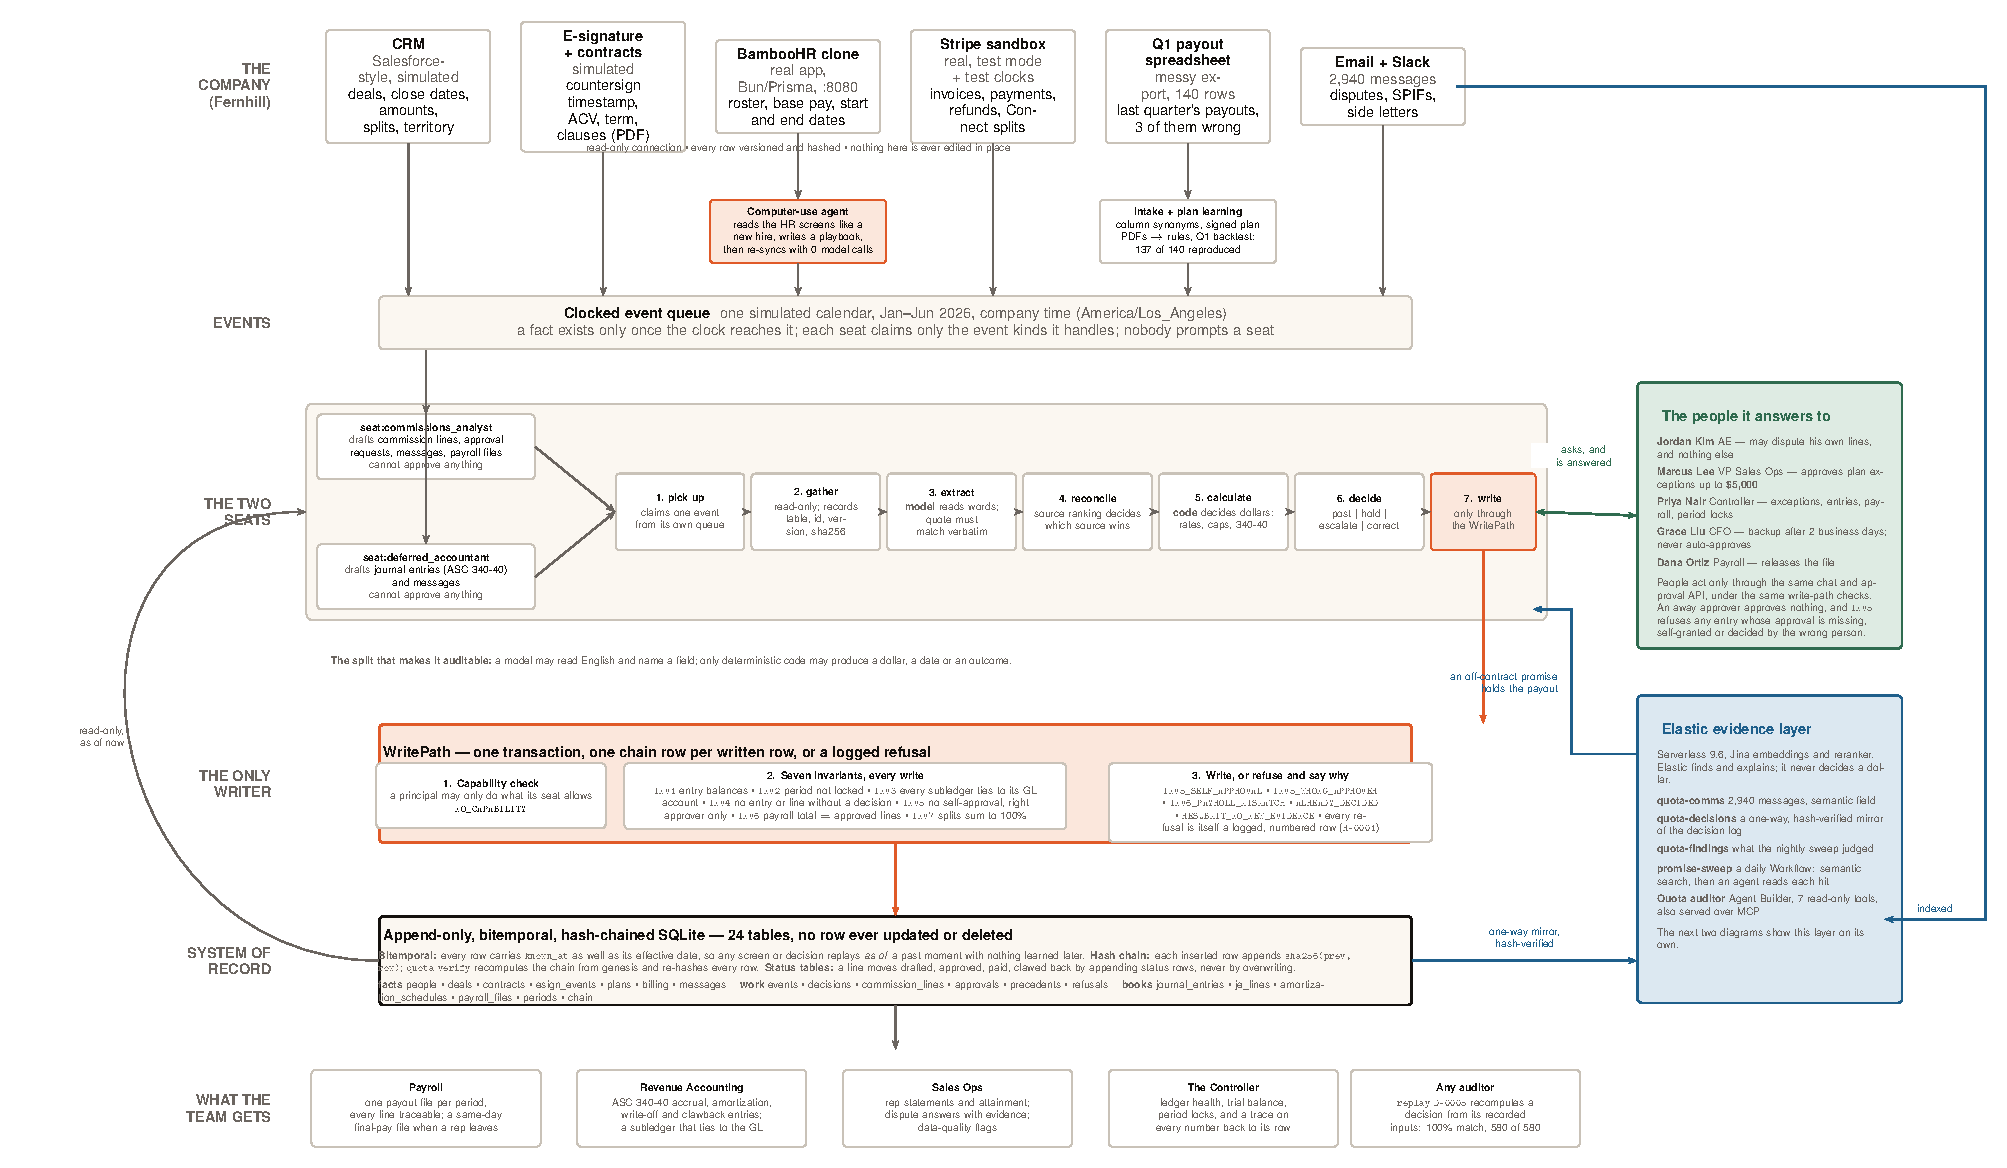
\includegraphics[width=\linewidth]{fig-architecture.pdf}
\end{center}
\end{landscape}

\begin{landscape}
\thispagestyle{empty}
\begin{center}
{\color{qblue}\large\bfseries Figure 2 \textemdash{} Elastic, 1 of 2: the promise sweep and the payout gate}\\[2pt]
\lead{How a sentence in an email becomes a \$6{,}000 hold, and the two code checks that stand between a model's reading and someone's paycheck.}\\[6pt]
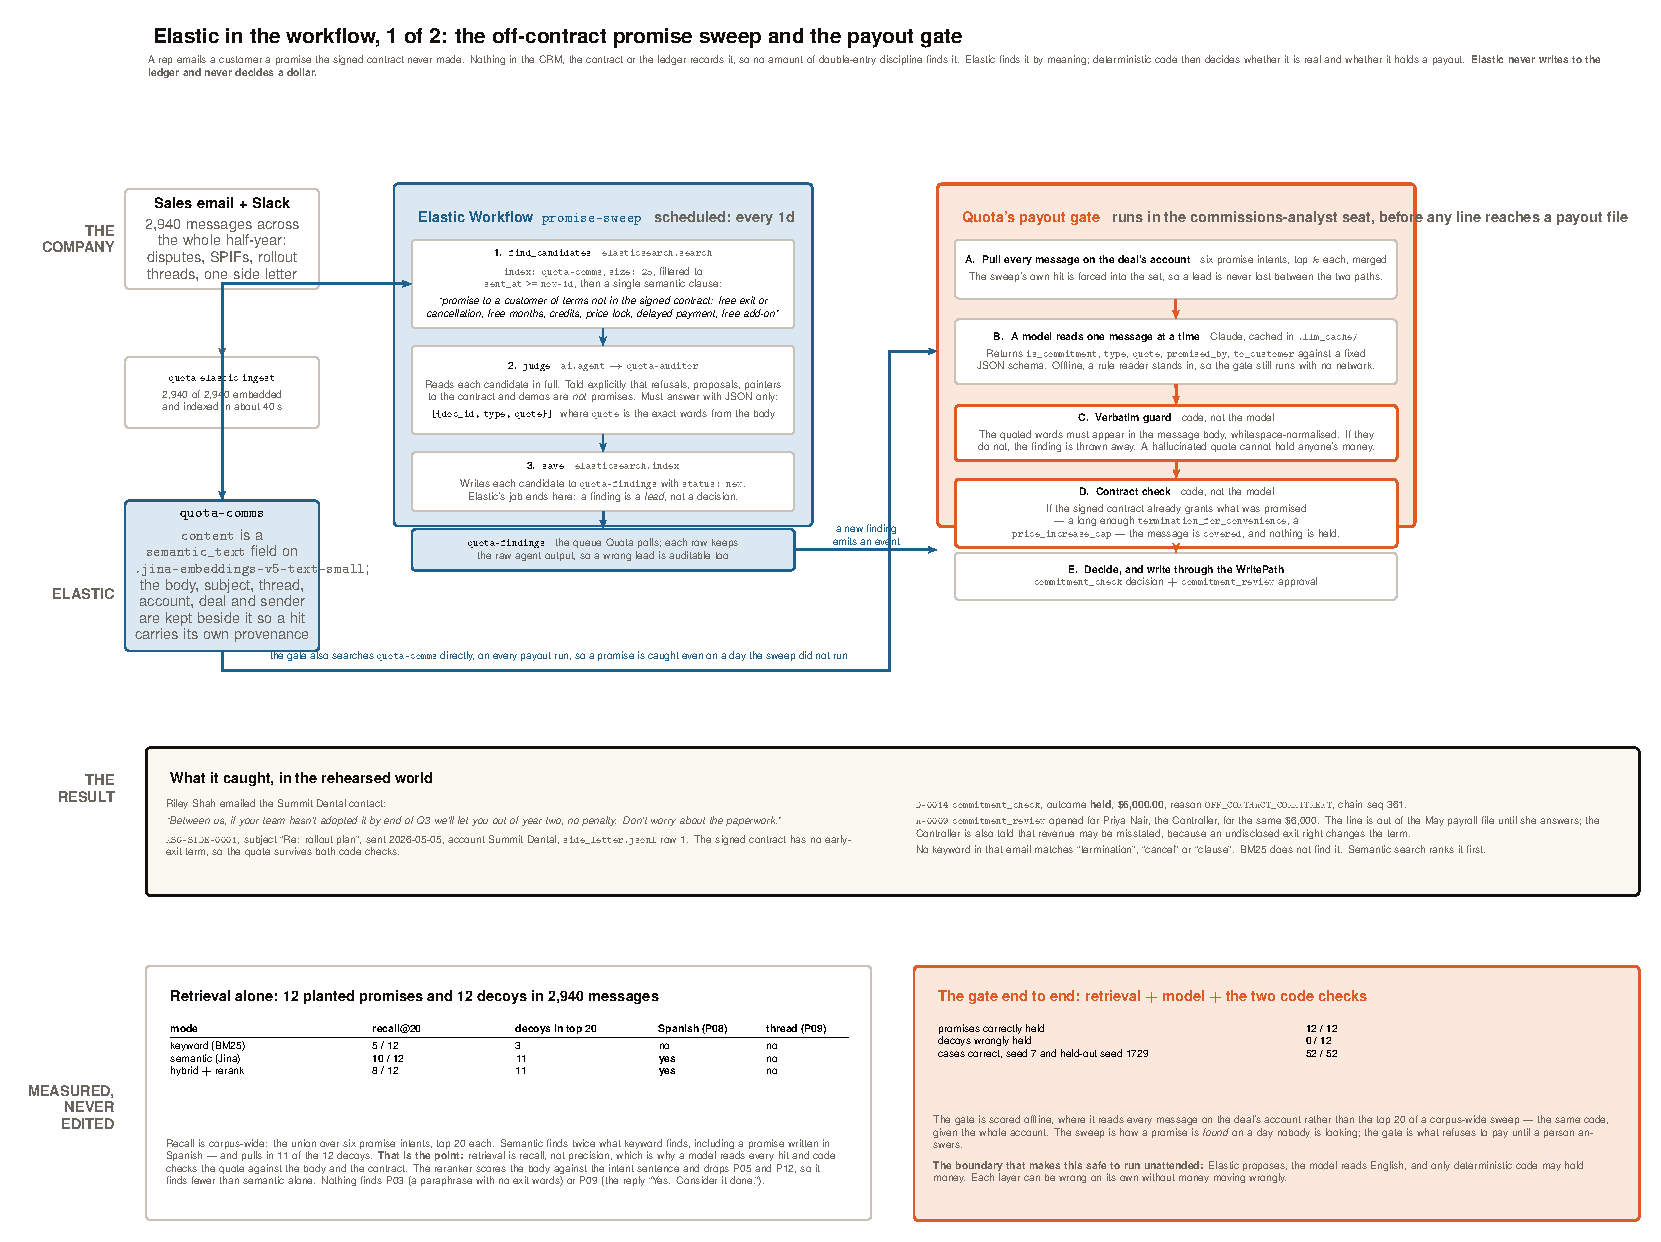
\includegraphics[width=\linewidth]{fig-elastic-sweep.pdf}
\end{center}
\end{landscape}

\begin{landscape}
\thispagestyle{empty}
\begin{center}
{\color{qblue}\large\bfseries Figure 3 \textemdash{} Elastic, 2 of 2: the decision mirror and the auditor}\\[2pt]
\lead{A one-way, hash-verified mirror of the decision log, seven read-only tools, and the live rehearsal \textemdash{} including the question it answered wrongly, and why.}\\[6pt]
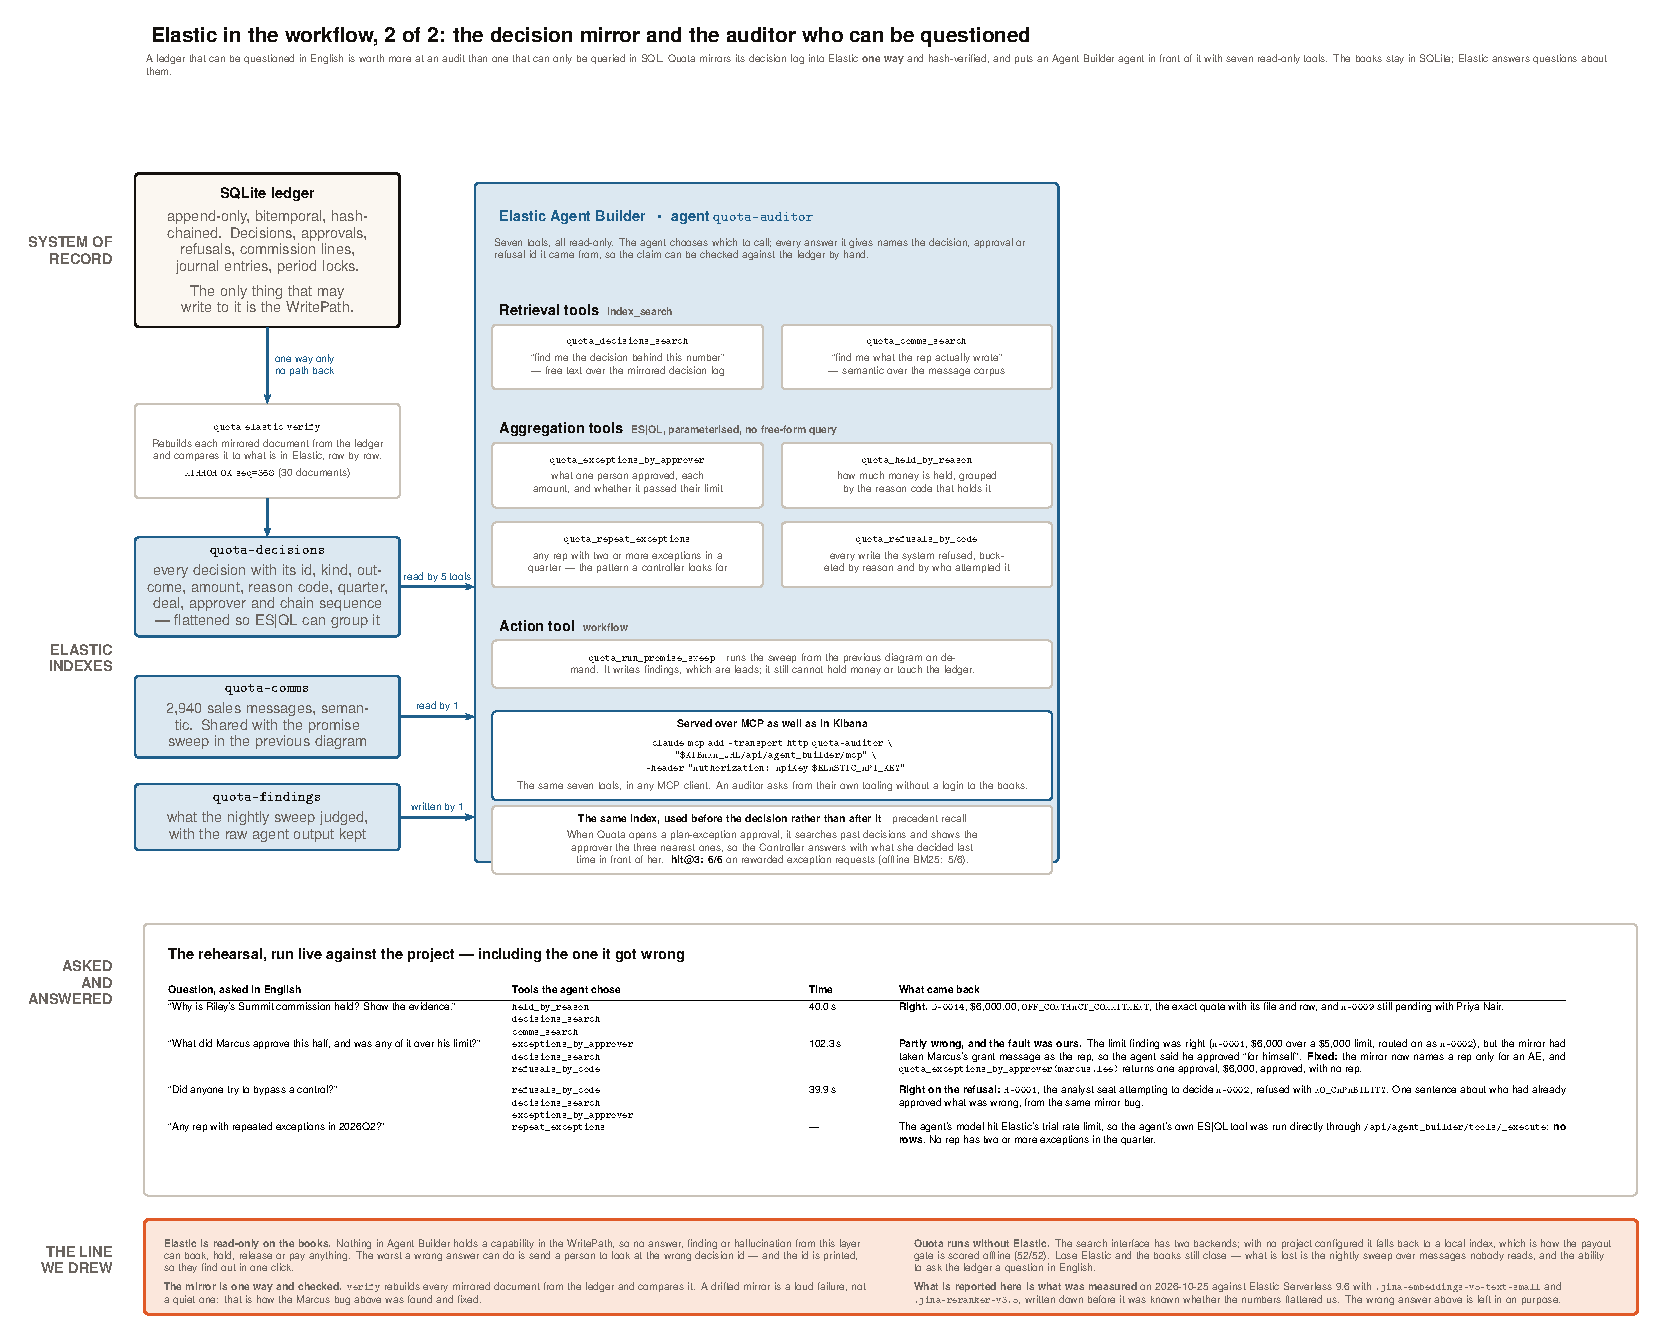
\includegraphics[width=\linewidth]{fig-elastic-auditor.pdf}
\end{center}
\end{landscape}

\end{document}
